\documentclass[xcolor=dvipsnames, USenglish]{beamer}  %notes=show to print them in the generated pdf
% Packages for a reasonable beamer session
\usepackage[T1]{fontenc}
%\usepackage[ansinew]{inputenc}
\usepackage[utf8]{inputenc}
\usepackage{textcomp}
\usepackage{lmodern}
\usepackage{csquotes}
\usepackage[english]{babel}
%\usepackage{babel}

\usepackage{graphicx}

\usepackage{amsmath}
\usepackage{amsfonts}
\usepackage{amssymb}
\usepackage{amsthm}
\usepackage{bm}

\usepackage{booktabs}
\usepackage{tabularx}

\usepackage{hyperref}

\usepackage{ellipsis}

% Additional packages
\usepackage{graphicx}
\usepackage{subfigure}
\usepackage{xcolor}
\usepackage{minted}

\usepackage[style=authoryear, backend=biber]{biblatex}
\setbeamertemplate{itemize/enumerate body begin}{\setlength{\leftmargini}{1.5em}}
\renewcommand*{\nameyeardelim}{\addcomma\addspace}
\addbibresource{\jobname.bib}
\renewcommand{\footnotesize}{\tiny}

\usepackage{tikz,pgf,calc}
%\usetikzlibrary{matrix, shapes, positioning, calc,
%  decorations.pathreplacing, shapes.geometric, arrows}
\usetikzlibrary{shapes.geometric, arrows, calc}
\tikzstyle{startstop} = [rectangle, rounded corners, minimum width=3cm, minimum height=1cm, text centered, text width=1.5cm, draw=black, fill=red!30]
\tikzstyle{io} = [trapezium, trapezium left angle=70, trapezium right angle=110, minimum width=3cm, minimum height=1cm, text centered, draw=black, fill=blue!30]
\tikzstyle{process} = [rectangle, minimum width=3cm, minimum height=1cm, text centered, draw=black, fill=orange!30]
\tikzstyle{decision} = [diamond, minimum width=3cm, minimum height=0.5cm, text centered, draw=black, fill=green!30]
\tikzstyle{arrow} = [thick,->,>=stealth]

%% References
\newlength\leftsidebar
\makeatletter
\setlength\leftsidebar{\beamer@leftsidebar}
\makeatother

\usepackage[absolute,overlay]{textpos}
\newenvironment{reference}[2]{%
  \begin{textblock*}{\textwidth}(\leftsidebar+#1,\paperheight-#2)
      \scriptsize\bgroup\color{red!50!black}}{\egroup\end{textblock*}}

% Path to graphics
\graphicspath{{../img/}}

% Sources
\usepackage{setspace}
\newcommand{\source}[1]{\begin{spacing}{0.5}{\fontsize{5}{6}\selectfont source: \itshape {#1}}\end{spacing}}
 % PACKAGES
% Collection of useful mathematical symbols and commands
% Calculus
\newcommand{\ud}{\mathrm{d}}
\newcommand{\pder}[2]{\frac{\partial{#1}}{\partial{#2}}}
\newcommand{\dpder}[2]{\frac{\partial^2{#1}}{\partial{#2^2}}}
\newcommand{\sderp}[3]{\frac{\partial^2{#1}}{\partial{#2}\partial{#3}}}
\newcommand{\tder}[2]{\frac{\ud{#1}}{\ud{#2}}}
\newcommand{\rot}[1]{\nabla \times {#1}}
\newcommand{\diver}[1]{\nabla \cdot {#1}}
\newcommand{\definter}[4]{\int_{#1}^{#2} {#3}\ud {#4}}
\newcommand{\inter}[2]{\int {#1}\ud {#2}}
\newcommand{\braket}[2]{\langle {#1} , {#2} \rangle}
% Misc
\newcommand{\eval}[1]{\Big |_{#1}}
\newcommand{\bset}[1]{\big\lbrace {#1} \big\rbrace}
\newcommand{\stimes}[2]{{#1}\!\times\!{#2}}
\newcommand{\trp}{\top}
\newcommand{\preup}[2]{{}^{#2}\!{#1}}

% Operators
\DeclareMathOperator*{\armin}{arg\,min}
\DeclareMathOperator*{\armax}{arg\,max}
\DeclareMathOperator*{\rank}{rank}
\DeclareMathOperator*{\cov}{cov}
\DeclareMathOperator*{\nullsp}{null}
% Logicals
\newcommand{\suchthat}{\big \backslash \;}
   % SYMBOLS

% ----------- extra packages
\usepackage{../beamer_themes/beamerthemeEawag_blue} % Eawag style

% ----------- Extra symbols
\newcommand{\ccov}[1]{{\color{red}k}\left(#1\right)}
\newcommand{\cmean}[1]{{\color{blue}m}\left(#1\right)}
\newcommand{\sm}{\scalebox{0.5}{-1}}

%----------------
% title information
\title{Master Thesis - Presentation 1}
\subtitle{Development of an Overland Flow Model Emulator}
\author[\texttt{sebastiano.rusca@eawag.ch}]{Sebastiano Rusca}
\institute[Eawag]{Eawag: Swiss Federal Institute of Aquatic Science
  and Technology}
\date[18.12.2017]{December 18, 2017}

% ====================================================================

\begin{document}

% ----------------
% Title frame
% load background for title
\setbeamertemplate{background}{
  
\includegraphics[width=\paperwidth,height=\paperheight]
  {../beamer_themes/background_title_blue.png}}
{ \setbeamertemplate{footline}{} % no footer on title
  \begin{frame}
    \titlepage
  \end{frame}
}
% load background for all other slides
\setbeamertemplate{background}{

\includegraphics[width=\paperwidth,height=\paperheight]
{../beamer_themes/background_slides_blue.png}}
\setbeamertemplate{footline}[Sebastiano Rusca] % set footer
\addtocounter{framenumber}{-1}  % don't count title page

%%%%%%%%%%%%%%%%%%%%%%%%%%%%%%%%%%%%%%%%%%%%%%%
%----------------
\section{Introduction}

  \begin{frame}
    \frametitle{Aim and Tasks}
    \begin{itemize}
      \item \textbf{Aim}: develop an overland flow model emulator for a concrete case study in Switzerland
      \item \textbf{Task 0}: get hands-on with the \emph{Shallow Water Equation}
      \item \textbf{Task 1}: channel flow simulations in FullSWOF2d
      \item \textbf{Task 2}: more complex simulations for which analytical
        solutions exists, e.g. dam break wave propagation
      \item \textbf{Final Task}: simulations of a concrete case study. Implement
        some mitigations measures. Optimize them with the help of the emulator
     \end{itemize}
     \note{I am trying to write some notes here}
  \end{frame}

%%%%%%%%%%%%%%%%%%%%%%%%%%%%%%%%%%%%%%%%%%%%%%%%%%%%%%%%%%%%%%%%%%%%%%%%%%%%%%%%
% TASK 0 - 1-D advection equation

\section{Task 0}

  \begin{frame}
    \frametitle{Task 0: 1-D advection equation}
    \centering
    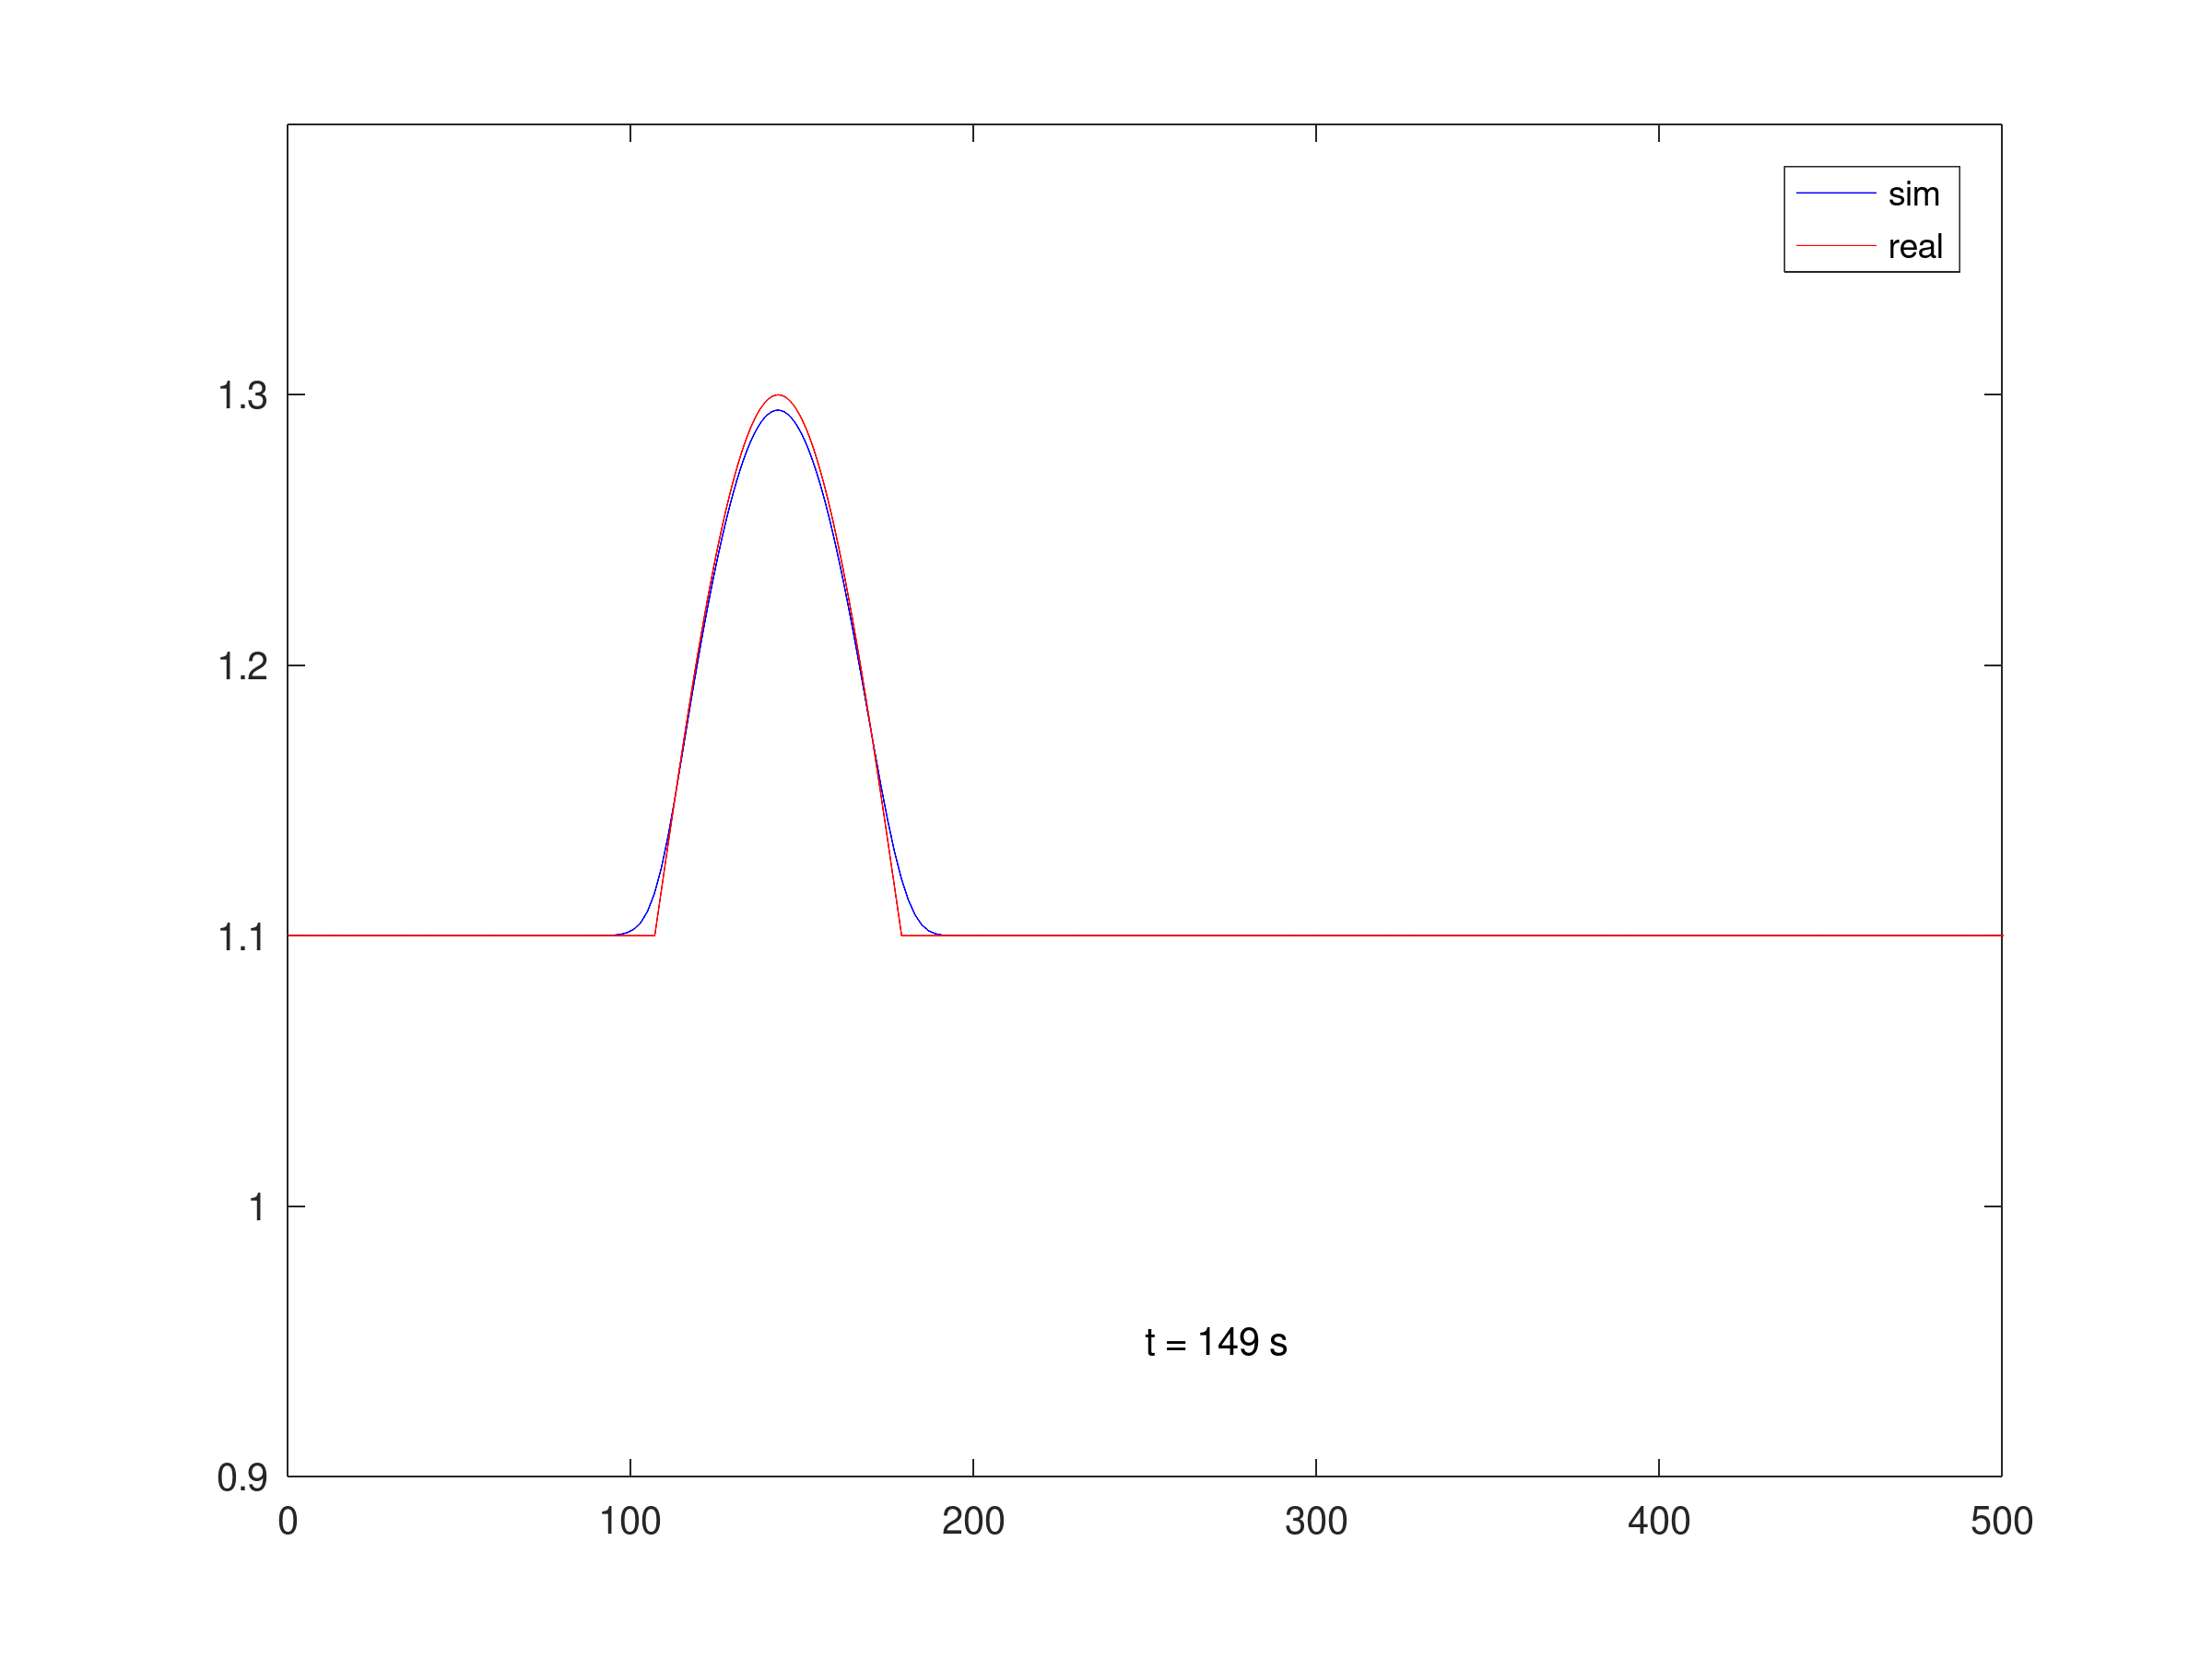
\includegraphics[width=0.8\textwidth]{img01/advection.eps}
  \end{frame}

%%%%%%%%%%%%%%%%%%%%%%%%%%%%%%%%%%%%%%%%%%%%%%%%%%%%%%%%%%%%%%%%%%%%%%%%%%%%%%%%
% TASK 1 - Setup

\section{Task 1}

  \begin{frame}
    \frametitle{Task 1: Channel simulations - Setup}
    \centering
    \includegraphics[width=0.6\textwidth]{img01/setup.eps}
    \note{another note here for this slide}
  \end{frame}

%%%%%%%%%%%%%%%%%%%%%%%%%%%%%%%%%%%%%%%%%%%%%%%%%%%%%%%%%%%%%%%%%%%%%%%%%%%%%%%%
% TASK 1 - Topography

\section{Task 1}

  \begin{frame}
    \frametitle{Task 1: Channel simulations - Topography}
    \centering
    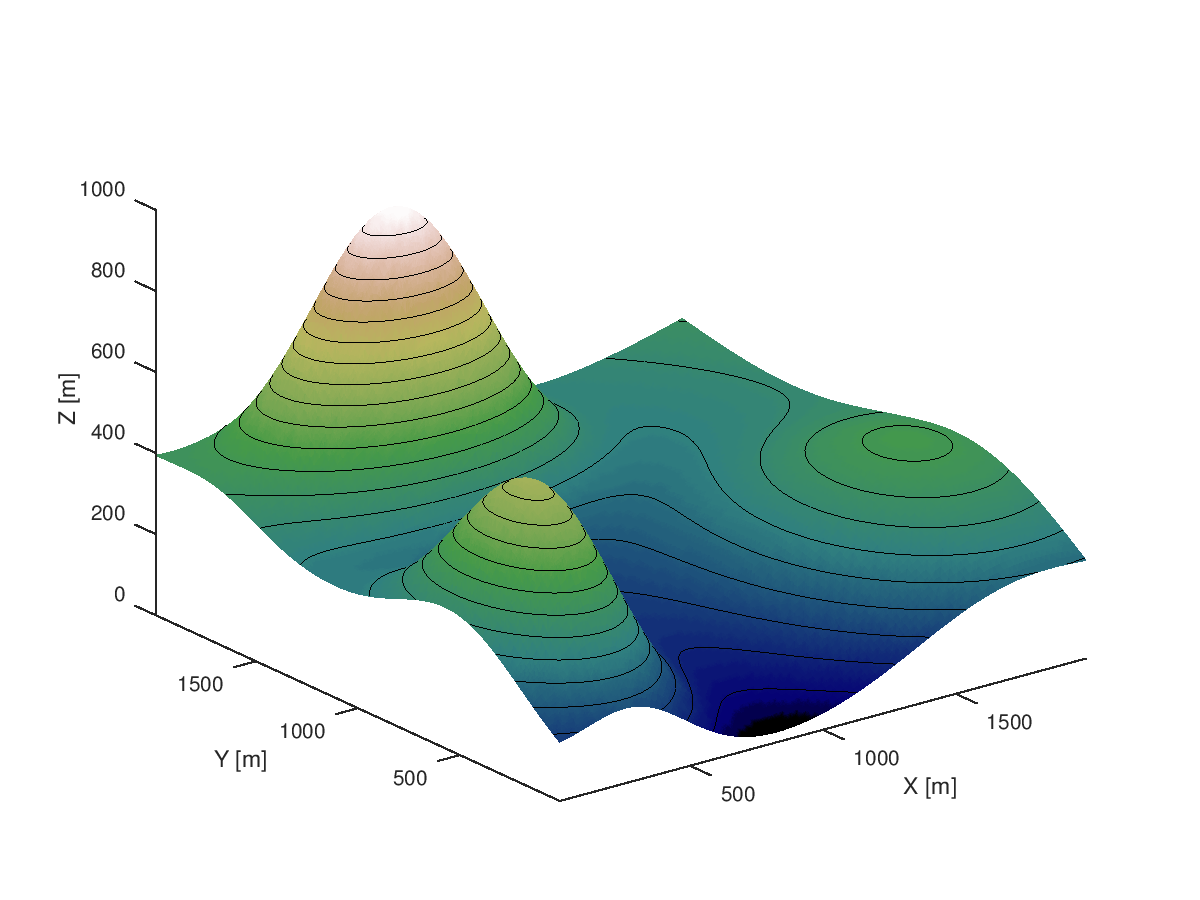
\includegraphics[width=0.8\textwidth]{img01/topography.eps}
  \end{frame}

%%%%%%%%%%%%%%%%%%%%%%%%%%%%%%%%%%%%%%%%%%%%%%%%%%%%%%%%%%%%%%%%%%%%%%%%%%%%%%%%
% Animation - Constant water depth channel experiment

\section{Animations}
  {
  \setbeamertemplate{background}{}
  \setbeamercolor{background canvas}{bg=black}
  \setbeamercolor{normal text}{fg=white}
  \usebeamercolor[fg]{normal text}
  \begin{frame}[plain]
    \centering
    \Large{\textbf{Animations:}}\\
    \begin{flushleft}
      \Large{-- Constant water depth channel experiment}\\
      \Large{-- Water bump in channel experiment}
    \end{flushleft}
  \end{frame}
  }

%%%%%%%%%%%%%%%%%%%%%%%%%%%%%%%%%%%%%%%%%%%%%%%%%%%%%%%%%%%%%%%%%%%%%%%%%%%%%%%%
% Next Phase

\section{Next Phase}

  \begin{frame}
    \frametitle{Next Phase: 1\textsuperscript{st} emulation step}
    \begin{itemize}
      \item Study effect of variation of one parameter for a specific case study
      \item Run simulations with different parameter values
      \item Generate Input -- Output plot
      \item Interpolate the values to obtain emulator for the chosen parameter
    \end{itemize}
  \end{frame}








%%%%%%%%%%%%%%%%%%%%%%%%%%%%%%%%%%%%%%%%%%%%%%%
%----------------
%\section{What is emulation?}
%  {
%  \setbeamertemplate{background}{}
%  \setbeamercolor{background canvas}{bg=black}
%  \setbeamercolor{normal text}{fg=white}
%  \usebeamercolor[fg]{normal text}
%  \begin{frame}[plain]
%    \centering
%    \Large{\textbf{What is emulation?}}\\
%    \Large{How is emulation even possible?}
%  \end{frame}
%  }

%  \begin{frame}{Alien researcher}
%    \centering
%    \begin{columns}[T]
%      \column{.5\textwidth}
%        \includegraphics[height=0.7\textheight]{molecule_spring.png}
%      \column{.5\textwidth}
%        \includegraphics[height=0.6\textheight]{HookesLaw.png}\\
%        \source{by Svjo, CC BY-SA 3.0, \url{commons.wikimedia.org/w/index.php?curid=25795521}}
%    \end{columns}
%  \end{frame}

%  \begin{frame}[t]{From molecules to fluids}
%    \centering
%    \only<1>
%    {
%      \href{run:../img/Pseudofluids_Chipmunk.avi?autostart&loop&noprogress}%
%       {\includegraphics[height=0.8\textheight]{pseudofluids.png}}
%    }
%    \only<2>
%    {
%      \includegraphics[height=0.75\textheight]{coarse_graining.png}\\
%      \source{doi:10.1088/0965-0393/12/6/R01}
%    }
%  \end{frame}

%  \begin{frame}{Emulation}
%  \framesubtitle{many names \& similarities ...}
%    \begin{tikzpicture}[overlay,remember picture,shift=(current page.north west)]
%      \pgfmathsetseed{4}
%      \foreach [count=\count] \word in {
%                                        Surrogate modeling,
%                                        Metamodeling,
%                                        Coarse graining,
%                                        Model order reduction,
%                                        Inter-polation,
%                                        Phenom. modeling,
%                                        Extra-polation,
%                                        Response surface,
%                                        Empiric. modeling
%                                       }
%      {
%        \pgfmathparse{round(70+20*rand)}
%        \edef\tr{\pgfmathresult}
%        \pgfmathparse{round(50+25*rand)}
%        \edef\tg{\pgfmathresult}
%        \pgfmathparse{round(50+50*rand)}
%        \edef\tb{\pgfmathresult}
%        \node [
%            anchor=west,
%            text width=2.5cm,
%            xshift=1.5cm,
%            yshift=-3cm,
%            xshift={mod(\count-1,3)*(\textwidth-2cm)/2},
%            yshift={floor((\count-1)/3)*(-(0.9\textheight-4cm))/2},
%            xshift=rand*2cm,
%            yshift=rand*1cm,
%            rotate=rand*15,
%            text={rgb:red,\tr;green,\tg;blue,\tb},
%            font=\bfseries\large] {\word};
%      }
%    \end{tikzpicture}

%  \end{frame}

%%%%%%%%%%%%%%%%%%%%%%%%%%%%%%%%%%%%%%%%%%%%%%%%
%%%----------------
%\section{Types of models}
%  {
%  \setbeamertemplate{background}{}
%  \setbeamercolor{background canvas}{bg=black}
%  \setbeamercolor{normal text}{fg=white}
%  \usebeamercolor[fg]{normal text}
%  \begin{frame}[plain]
%    \centering
%    \Large{\textbf{Types of simulators}}
%  \end{frame}
%  }

%  \input{../includes/models.tex}

%  \begin{frame}{Combination of models}
%    \framesubtitle{Dimensional heterogeneous models}

%    \begin{columns}[c]
%      \column{0.5\textwidth}
%        \centering
%        \includegraphics[height=0.4\textheight]{heterogeneous_hemo.png}\\
%        \includegraphics[height=0.4\textheight]{crack3D.png}

%      \column{0.5\textwidth}
%        {\small
%        \begin{itemize}
%        \item Some details are less relevant
%        \item "Simplify" those
%          \begin{itemize}
%          \item 1D phenomenological
%          \item 1D Emulator of detailed model
%          \item Reduced model
%          \end{itemize}
%        \item Coupling is challenging
%        \end{itemize}
%        }
%    \end{columns}

%  \end{frame}

%%%%%%%%%%%%%%%%%%%%%%%%%%%%%%%%%%%%%%%%%%%%%%%%
%%%----------------
%\section{Speeding up simulators}
%  {
%  \setbeamertemplate{background}{}
%  \setbeamercolor{background canvas}{bg=black}
%  \setbeamercolor{normal text}{fg=white}
%  \usebeamercolor[fg]{normal text}
%  \begin{frame}[plain]
%    \centering
%    \Large{\textbf{Speeding-up simulators}}
%  \end{frame}
%  }

%  \begin{frame}{Numerical models: common scenarios}
%    \begin{columns}[c]
%      \column{.5\textwidth}
%        \includegraphics[width=\textwidth]{example1.png}

%      \column{.5\textwidth}
%      \begin{enumerate}
%        \item Inputs (several):
%          \begin{itemize}
%            \item Rain, e.g. Hyetograph
%            \item Initial water levels
%            \item Pipe parameters
%            \item \dots
%          \end{itemize}
%        \item Internal states (many)
%        \item Outputs (few):
%          \begin{itemize}
%            \item Water level or flow at marked outlet
%          \end{itemize}
%      \end{enumerate}
%    \end{columns}
%  \end{frame}

%  \begin{frame}{Numerical models: common scenarios}
%    \framesubtitle{Fan-out, fan-in}
%    \centering
%    \includegraphics[width=0.8\textwidth]{FanOutIn.png}
%  \end{frame}

%  \begin{frame}[t]{Simulation speed-up tools?}
%    \alert{Simulation-hungry} applications are common.
%    What can we do?

%    \begin{columns}[t]
%      \column{0.5\textwidth}
%        \begin{block}{Model order reduction (MOR)}
%        New model with fewer states approximates original model, e.g. reduced basis methods, balanced truncation, cross Gramian, \ldots
%        \footnote{\url{morwiki.mpi-magdeburg.mpg.de}}
%        \end{block}
%      \column{0.5\textwidth}
%        \begin{block}{Emulation}
%          Use input-output data to build an interpolant, e.g. Gaussian processes, neural networks, polynomial expansions, \ldots

%          Can use details of the original model.
%        \end{block}
%    \end{columns}
%    \vspace{1em}
%    There is a gamut from emulation to MOR.

%    Emulation $=$ extreme MOR.

%    Emulation is "simpler" than MOR.
%  \end{frame}

%  \begin{frame}{Model order reduction}
%    \centering
%    \only<1>{\includegraphics[width=0.8\textwidth]{FanOutIn.png}}
%    \only<2>{
%      \includegraphics[width=0.8\textwidth]{MOR.png}

%      Internal states can be recovered (aprox.)
%    }
%    \only<3>{
%      \includegraphics[width=0.8\textwidth]{Snapshots.png}\\
%      \includegraphics[width=0.6\textwidth]{Manifold.png}\\
%      \vspace{-1em}\flushleft\source{Quarteroni et al.(2016), ISBN 978-3-319-15430-5, Springer}
%    }
%  \end{frame}

%  \begin{frame}{Emulation}
%    \framesubtitle{TIMTOWTDI}
%    \centering
%    \only<1>{\includegraphics[width=0.8\textwidth]{FanOutIn.png}}
%    \only<2>{
%      \includegraphics[width=0.8\textwidth]{EmulationIdea.png}
%    }
%    \onslide<2>{
%      Internal states are lost

%      Another name: Input-Output relations of complex nonlinear systems (linear case: \emph{transfer functions})
%    }
%  \end{frame}

%%%%%%%%%%%%%%%%%%%%%%%%%%%%%%%%%%%%%%%%%%%%%%%%
%%%----------------
%\section{When is emulation useful?}
%  {
%  \setbeamertemplate{background}{}
%  \setbeamercolor{background canvas}{bg=black}
%  \setbeamercolor{normal text}{fg=white}
%  \usebeamercolor[fg]{normal text}
%  \begin{frame}[plain]
%    \centering
%    \Large{\textbf{When is emulation (not) useful?}}
%  \end{frame}
%  }

%  \begin{frame}{Define your task}
%    \framesubtitle{no task, no emulator}

%    Applications:
%    \begin{itemize}
%      \item Real-time control (if optimal then includes optimization)
%      \item Optimization
%      \begin{itemize}
%        \item System identification (a.k.a. model calibration)
%        \item Preliminary and detailed engineering design (\alert{conceptual design?})
%        \item Experimental design
%      \end{itemize}
%      \item Real-time vizualization \& feedback ((serious) games)
%      \item \dots
%    \end{itemize}
%  \end{frame}

%  \begin{frame}{Model predictive realtime control}
%    \only<2-5>{
%      \begin{tikzpicture}
%        \node[anchor=south west,inner sep=0] (image) at (0,0) {\includegraphics[width=\textwidth]{model_predictive.png}};
%        \begin{scope}[x={(image.south east)},y={(image.north west)}]
%          \only<2>{\fill[white] (0.3,0) rectangle (1,1);}
%          \only<3>{\fill[white] (0.529,0) rectangle (1,1);}
%          \only<4>{\fill[white] (0.756,0) rectangle (1,1);}
%        \end{scope}
%      \end{tikzpicture}
%   }
%   \only<1>{
%    \vspace{-2em}
%    \centering
%    \includegraphics[width=\textwidth]{Network_Water.png}\\
%    \vspace{-2em}\flushleft\source{RTC4Water}\hfill

%    \begin{columns}[t]
%      \column{.3\textwidth}
%        1. Measure current state
%      \column{.4\textwidth}
%        2. \alert{Optimize} decisions based on prediction of future states
%      \column{.3\textwidth}
%        3. Recalibrate model
%    \end{columns}
%   }
%  \end{frame}

%  \begin{frame}{System identification}
%    \begin{columns}
%      \column{.5\textwidth}
%        \includegraphics[width=\textwidth]{f4.png}\\
%        \vspace{-1em}\source{GPML toolbox}

%      \column{.5\textwidth}
%        \begin{enumerate}
%          \item Get data
%          \item \alert{Find} model parameters values (distributions) consistent with data. Loads of simulations!
%        \end{enumerate}
%    \end{columns}
%  \end{frame}

%  \begin{frame}{Design}
%    \vspace{-0.8em}
%    \centering
%    \includegraphics[height=0.8\textheight]{emu_design.png}\\
%    \source{H Zhong-Hua \& K-S Zhang. "Surrogate-based optimization". InTech, 2012.}
%  \end{frame}

%%%%%%%%%%%%%%%%%%%%%%%%%%%%%%%%%%%%%%%%%%%%%%%%
%%%----------------
%\section{Learning from data}
%  {
%  \setbeamertemplate{background}{}
%  \setbeamercolor{background canvas}{bg=black}
%  \setbeamercolor{normal text}{fg=white}
%  \usebeamercolor[fg]{normal text}
%  \begin{frame}[plain]
%    \centering
%    \Large{\textbf{Learning from data}}\\
%    \Large{Machine learning (supervised)}
%  \end{frame}
%  }

%  \input{../includes/learning_from_data.tex}


%  \begin{frame}[t]{Interpolation}
%    \framesubtitle{Curse of dimensionality (polynomials)}
%    Take $m$ 1-D data points. What's the "simplest" (degree) polynomial that inteprolates the data?
%    \pause
%    
%    Degree $m+1$, regardless of where they are (not repeated).
%    \pause

%    \vspace{1em}
%    What about with $m$ d-D data points?
%    \pause 
%    
%    $d>2$ there isn't unless the position is specified ($\pi_m(\mathbb{R}^d)$-\emph{unisolvent}), e.g. (perturbed) grids.

%  \begin{reference}{2mm}{2em}
%   Wendland, H. (2004). Scattered data approximation (Vol. 17). Cambridge university press. Ch. 2.
%  \end{reference}

%  \end{frame}

%  \begin{frame}[t]{How many samples?}
%  If $m$-degree polynomial interpolation on $d$-dimensional grid:

%  \begin{gather*}
%    N = \begin{pmatrix}m + d \\ d\end{pmatrix}\\
%    m = 7, d = 3 \rightarrow N = 120
%  \end{gather*}

%  \begin{reference}{2mm}{2em}
%   Wendland, H. (2004). Scattered data approximation (Vol. 17). Cambridge university press. Ch. 2.
%  \end{reference}
%  \end{frame}

%%%%%%%%%%%%%%%%%%%%%%%%%%%%%%%%%%%%%%%%%%%%%%%%
%%%----------------
%\section{pre-Emulation}
%  {
%  \setbeamertemplate{background}{}
%  \setbeamercolor{background canvas}{bg=black}
%  \setbeamercolor{normal text}{fg=white}
%  \usebeamercolor[fg]{normal text}
%  \begin{frame}[plain]
%    \centering
%    \Large{\textbf{Before jumping into emulation}}
%  \end{frame}
%  }

%  \begin{frame}{Nondimensional models}
%    \framesubtitle{A simple example: pendulum}

%    Equation of motion of a pendulum:
%    \[
%      \ell\tder{{}^2\theta}{t^2} + g\sin \theta = 0
%    \]
%    How many parameters?

%    We know it will oscillate... is the period $T$ a function of the parameters?
%    $[T] = s$, $[g]=\frac{m}{s^2}$ and $[\ell] = m$ then
%    \[
%      T \sim \sqrt{\frac{l}{g}}
%    \]
%    This property of the oscillations depends on a single parameter: the ratio $l/g$.

%    Check <somebody> number and  Buckingham $\pi$ theorem.

%  \end{frame}

%  \begin{frame}{Exploratory data analysis}
%    \begin{itemize}
%      \item Prior knowledge about the process?
%      \item Function from inputs to outputs?
%      \item All inputs relevant?
%      \item Reduced dimension?
%      \item Stationary or not?
%      \item Do I need a fancy method?
%    \end{itemize}
%  \end{frame}
%%%%%%%%%%%%%%%%%%%%%%%%%%%%%%%%%%%%%%%%%%%%%%%%
%%%----------------
%\section{Summary}
%  {
%  \setbeamertemplate{background}{}
%  \setbeamercolor{background canvas}{bg=black}
%  \setbeamercolor{normal text}{fg=white}
%  \usebeamercolor[fg]{normal text}
%  \begin{frame}[plain]
%    \centering
%    \Large{\textbf{Summary}}
%  \end{frame}
%  }

%  \begin{frame}[t]{Recap}
%    \centering
%    \begin{itemize}
%      \item General simulators $\notin$ simulation intensive applications
%      \item Speed-up: general vs. specific (fan-out $\rightarrow$ fan-in)
%      \item Detail vs. speed tradeoff is relaxed via emulation/MOR
%      \item If general simulators needed (internal states) $\rightarrow$ MOR
%      \item If specific problem with "low dimensional" output $\rightarrow$ Emulation
%      \item Define task $\rightarrow$ define emulation strategy
%      \item Prefer methods that allocate your knowledge about the process
%        \begin{itemize}
%          \item "Better" extrapolation! (interpretable, foreseeable, \dots)
%          \item Lower demand on data
%        \end{itemize}
%    \end{itemize}
%  \end{frame}

%  \begin{frame}
%    \frametitle{pre-Emulation flowchart}
%    \begin{center}
%    \begin{tikzpicture}[node distance=2cm]

%    \node (problem)[startstop]{Task: DoE, SI, RTC, \dots};
%    \node (model)[decision, right of=problem,xshift=2cm]{Model};
%    \node (modeling)[process, right of=model, xshift=2cm]{Build a model};
%    \node (dataset)[decision, yshift=-0.5cm, below of=model]{Dataset};
%    \node (dataseting)[process, right of=dataset, xshift=2cm]{Assemble dataset};
%    \node (stop)[startstop, below of=dataset, yshift=-0.5cm]{Emulate};

%    \draw [arrow] (problem) -- (model);
%    \draw [arrow] (model) -- node[anchor=south]{no} (modeling);
%    \draw [arrow] (model) -- node[anchor=east]{yes} (dataset);
%    \draw [arrow] (dataset) -- node[anchor=south]{no} (dataseting);
%    \draw [arrow] (dataset) -- node[anchor=east]{yes} (stop);
%    \draw [arrow] (modeling) -- (dataseting);
%    \draw [arrow] (dataseting) |- (stop);

%    \end{tikzpicture}
%    \end{center}
%  \end{frame}



%%%%%%%%%%%%%%%%%%%%%%%%%%%%%%%%%%%%%%%%%%%%%%%%
%%%----------------
%\section{Resources}
%  {
%  \setbeamertemplate{background}{}
%  \setbeamercolor{background canvas}{bg=black}
%  \setbeamercolor{normal text}{fg=white}
%  \usebeamercolor[fg]{normal text}
%  \begin{frame}[plain]
%    \centering
%    \Large{\textbf{Resources}}\\
%    \small{\url{https://bitbucket.org/KaKiLa/emumore/wiki/Resources.md}}\\
%    \Large{Inputs welcomed!}
%  \end{frame}
%  }

%%%%%%%%%%%%%%%%%%%%%%%%%%%%%%%%%%%%%%%%%%%%%%%%
%%%----------------
%\section{Conclusion}
%  {
%  \setbeamertemplate{background}{}
%  \setbeamercolor{background canvas}{bg=black}
%  \setbeamercolor{normal text}{fg=white}
%  \usebeamercolor[fg]{normal text}
%  \begin{frame}[plain]
%    \centering
%    \Large{\textbf{Thank you!}}\\
%    \Large{\textbf{Q \& A}}\\
%    \vfill
%    \small{
%    There is a table reserved for lunch.

%    Afternoon session begins at 14:00.

%    Registered participants: closure apero (\textasciitilde 17:00)!
%    }
%  \end{frame}
%  }

\end{document}

